\documentclass[lettersize,journal]{IEEEtran}
\usepackage{amsmath,amsfonts,amssymb,amsthm}
\usepackage{algorithm}
\usepackage{algpseudocode}
\usepackage{array}
\usepackage[caption=false,font=footnotesize,labelfont=rm,textfont=rm]{subfig}
\usepackage{textcomp}
\usepackage{stfloats}
\usepackage{url}
\usepackage{booktabs}
\usepackage{multirow}
\usepackage{graphicx}
\usepackage{cite}
\usepackage{xcolor}
\usepackage{pgfplots}
\pgfplotsset{compat=1.17}
\usepgfplotslibrary{groupplots}
\definecolor{navy}{HTML}{011E4B}
\definecolor{gold}{HTML}{FAB001}
\definecolor{sky}{HTML}{87C6E9}
\definecolor{alert}{HTML}{EE1C23}
\newtheorem{proposition}{Proposition}
\newtheorem{definition}{Definition}
\newtheorem{remark}{Remark}
\hyphenation{op-tical net-works semi-conduc-tor IEEE-Xplore}
\newcommand{\VicAccR}{89.9}
\newcommand{\VicAccV}{89.3}
\newcommand{\MaskBitsPerCoord}{0.0072}
\newcommand{\MaskBitsImage}{118}
\newcommand{\MaskBitsRhoK}{0.012}
\newcommand{\ExMinAgreeK}{99.98}
\newcommand{\ExMinAgreeTenK}{99.91}
\newcommand{\ExMaxRelErrHundred}{1.2\times10^{-5}}
\newcommand{\ExMaxRelErr}{1.2\times10^{-3}}
\newcommand{\OrigMsR}{3.25}
\newcommand{\OrigMsV}{4.99}
\newcommand{\StealScratchR}{70.1}
\newcommand{\StealPlainR}{74.4}
\newcommand{\StealGhostR}{68.2}
\newcommand{\StealBestGhostR}{71.2}
\newcommand{\StealGapR}{1.1}
\newcommand{\StealPsArrowR}{70.5}
\newcommand{\StealLeftProjR}{70.2}
\newcommand{\PubPublic}{86.6}
\newcommand{\PubPlain}{86.4}
\newcommand{\PubPsArrow}{86.7}
\newcommand{\PubBestGhost}{86.8}
\newcommand{\StealScratchV}{73.0}
\newcommand{\StealPlainV}{80.0}
\newcommand{\StealGhostV}{71.5}
\newcommand{\StealArrowV}{72.8}
\newcommand{\PubPsArrowErr}{0.029}
\newcommand{\PubLeftProjErr}{0.041}
\newcommand{\PubArrowErr}{1.145}
\newcommand{\PubUnmixErr}{2.789}
\newcommand{\PubProjKErr}{0.041}
\newcommand{\VicAccFt}{90.6}
\newcommand{\InvPsnrFirstZero}{37.2}
\newcommand{\InvPsnrFirstTen}{13.4}
\newcommand{\InvPsnrMean}{12.7}
\newcommand{\IcaRefErr}{0.065}
\newcommand{\IcaTrueB}{0.038}
\newcommand{\IcaBestErr}{0.329}
\newcommand{\IcaCin}{16}


\begin{document}
\title{GHOST: Guarded Hybrid Obfuscation with Split Token Execution for Secure Edge Inference}
\author{Siddharath~Malavalli~Nagesh,
        Mohamed~Firas~Adil,
        Rochishnu~Banerjee,
        Angel~Arul~Jothi~Joseph,
        and~Elakkiya~Rajasekar,~\IEEEmembership{Member,~IEEE}%
\thanks{S. Malavalli Nagesh, A. Arul Jothi Joseph, and E. Rajasekar are with the
Department of Computer Science, Birla Institute of Technology and Science,
Pilani, Dubai Campus, Dubai International Academic City, Dubai, United Arab
Emirates (e-mail: f20220224@dubai.bits-pilani.ac.in;
angeljothi@dubai.bits-pilani.ac.in; elakkiya@dubai.bits-pilani.ac.in).}%
\thanks{M. Firas Adil is with the EQS Department, Siemens Energy,
Side Quarter A, Expo City, Dubai, United Arab Emirates
(e-mail: Mohamedfirasadil@gmail.com; Mohamed.adil.ext@siemens-energy.com).}%
\thanks{R. Banerjee is with the Department of Computer Science and
Software Engineering, Miami University, Oxford, OH, USA
(e-mail: banerjr2@miamioh.edu).}%
\thanks{Corresponding author: E. Rajasekar.}%
}
\markboth{IEEE Transactions on Information Forensics and Security}%
{Malavalli Nagesh \MakeLowercase{\textit{et al.}}: GHOST: Guarded Hybrid Obfuscation with Split Token Execution}
\maketitle

\begin{abstract}
A convolutional neural network deployed on an edge device is exposed to the owner of that device through three channels: the weights held in device memory, the intermediate operands produced during inference, and the query interface. Defences based on trusted execution environments (TEEs) either keep most of the network inside the enclave, which is slow, or outsource linear layers to the untrusted processor under a weight obfuscation that recent direction-matching attacks have shown to be recoverable. These defences also treat unrestricted querying as outside their scope. This paper presents GHOST, a TEE-anchored design that addresses the three channels together. GHOST stores each edge convolution as a two-sided mixing of its filters and of random decoy filters, releases only channel-mixed activations under fresh one-time masks, executes the edge prefix only for queries that carry a valid authorisation token within a query budget, and keeps the suffix of the network in the cloud behind an authenticated encrypted channel. The construction is exact: at the default mask ratio the protected ResNet-20 and VGG-11 reproduce the unprotected predictions on every CIFAR-10 test input. Against an adversary who reads all untrusted memory and holds the checkpoint from which the victim was fine-tuned, direction matching and least-squares un-mixing recover nothing beyond that checkpoint, whereas direction matching recovers a permute-and-scale ablation to below the checkpoint's own error. Blind estimation of the input mixing from the released operands identifies its rows only when the effective mask ratio is low, at $\rho=1$ or when the mask is averaged out by repeated queries, which the mask ratio and the query budget control, and the recovered filters then remain five times further from the victim than the checkpoint. Masked operands reduce input reconstruction to close to the level of an uninformed guess, query-based extraction is capped by the TEE-enforced budget, and the work of the TEE per query is reported in operations and measured time for each split point.
\end{abstract}

\begin{IEEEkeywords}
Edge AI security, trusted execution environment, model stealing, weight obfuscation, split inference, model extraction, membership inference.
\end{IEEEkeywords}

\section{Introduction}
\label{sec:intro}
\IEEEPARstart{C}{onvolutional} neural networks (CNNs) are increasingly executed on the device that captures the data, for reasons of latency, bandwidth and privacy. A model deployed in this way is exposed to whoever controls the device. An adversary with control of the operating system can read the weights from memory and copy the model, observe intermediate activations and reconstruct the inputs of other users, and submit queries in order to train a functional surrogate~\cite{tramer2016stealing,orekondy2019knockoff} or to infer whether a record was part of the training set~\cite{shokri2017membership,carlini2022lira}. These three channels, namely device memory, intermediate operands and the query interface, are open at the same time, and an effective defence has to close all of them.

Hardware trusted execution environments (TEEs) such as Arm TrustZone~\cite{pinto2019trustzone} isolate a small amount of memory and computation from the rest of the device. Executing the entire network inside the TEE protects the weights but is limited by enclave memory and by the absence of accelerators~\cite{mo2020darknetz}. TEE-shielded partitioning places only selected layers inside the enclave~\cite{mo2020darknetz,zhang2024nplo}, and obfuscation-based outsourcing transforms the weights of linear layers so that the untrusted processor can execute them while the TEE restores the result~\cite{tramer2018slalom,sun2023shadownet,shen2022soter,zhang2024groupcover,sun2025tsqp}. Two lines of recent work show the limits of these designs. Partitioning schemes leak enough of the model for fine-tuning attacks to recover it~\cite{zhang2024nplo}, and obfuscation by permutation and scaling preserves the direction of every weight vector, which allows a direction-matching attack to recover the permutation from a public reference model~\cite{wang2025arrows}. In addition, the obfuscation-based designs explicitly exclude the query interface from their threat model~\cite{sun2023shadownet,mao2025amulet}, so a device owner can still extract the model through unlimited queries.

This paper presents GHOST (Guarded Hybrid Obfuscation with Split Token Execution), a design in which every protection is anchored in the TEE and the three exposure channels are addressed together. The edge prefix of the network is outsourced to the untrusted processor in a form that is exact, so the protected model computes the same function as the original. The weights of each edge convolution are stored only as a two-sided mixing of the real filters and of random decoy filters, which changes the direction of every stored vector and adds to each a random component. Activations leave the TEE only after channel mixing and a fresh one-time mask. The TEE executes the prefix only for requests that carry a valid authorisation token within a query budget, and the suffix of the network never reaches the device.

The contributions of this paper are as follows.
\begin{itemize}
\item An exact four-tier construction for TEE-anchored edge inference is presented that combines two-sided weight mixing with decoy filters, one-time masking of mixed activations, token-gated execution with replay protection and a query budget, and split edge-cloud execution behind an authenticated encrypted channel.
\item A threat model covering device memory, intermediate operands and the query interface is formalised, together with an exactness result, an information-theoretic bound on the leakage of masked operands, and a bound on the number of queries that the adversary can obtain.
\item An adaptive evaluation is carried out in which the adversary applies direction matching, least-squares un-mixing and row-space projection to the stored tensors, using its own model, an independently trained model on the victim's data, or the checkpoint from which the victim was fine-tuned as the reference, and is compared with permute-and-scale and left-only ablations.
\item The cost of the construction and its effect on model stealing are measured on ResNet-20 and VGG-11 for CIFAR-10, its effect on input reconstruction, query-based extraction and membership inference on ResNet-20, and the implementation, the attack suite and the scripts that produce every table and figure are released at \url{https://github.com/Elakkiya16/GHOST}.
\end{itemize}

\section{Related Work}
\label{sec:related}

\subsection{TEE Execution and TEE-Shielded Partitioning}
DarkneTZ~\cite{mo2020darknetz} executes the last layers of a network inside Arm TrustZone and the remaining layers in the untrusted environment. The layers outside the enclave are exposed in plaintext, and the protection therefore depends on how much of the model is shielded. A systematic evaluation of TEE-shielded partitioning~\cite{zhang2024nplo} showed that an adversary who combines the exposed layers with a small public dataset can fine-tune a surrogate that approaches the victim, and proposed TEESlice, which separates privacy-sensitive weights before training. These schemes protect the weights inside the enclave but leave the exposed layers and the query interface unprotected. GHOST exposes no plaintext weights on the device, keeps the suffix of the network in the cloud, and controls the query interface.

\subsection{Obfuscation-Based Outsourcing}
Slalom~\cite{tramer2018slalom} outsources linear layers from an SGX enclave to an untrusted GPU and hides the inputs with precomputed additive blinding factors, with the purpose of protecting input privacy and verifying integrity for a model that is not secret. ShadowNet~\cite{sun2023shadownet} protects model weights on TrustZone devices by scaling each filter, adding random noise filters and shuffling the filters, and it blinds the input of each outsourced layer with a fresh mask whose convolution is precomputed in the TEE. SOTER~\cite{shen2022soter} morphs the parameters of associative operators, NNSplitter~\cite{zhou2023nnsplitter} publishes a deliberately degraded copy of the weights and keeps the modified entries in the TEE, GroupCover~\cite{zhang2024groupcover} strengthens the randomness of the obfuscation, and TSQP~\cite{sun2025tsqp} targets quantised networks. The direction-matching attack of~\cite{wang2025arrows} recovers the permutation of five such schemes with more than 99\% accuracy whenever a public pre-trained model is available, because per-vector permutation and scaling leave vector directions unchanged, and~\cite{wang2025arrows} proposes mixing weight columns as a countermeasure. Amulet~\cite{mao2025amulet} masks linear weights on both sides with secret matrices, and MirageNet~\cite{zheng2026miragenet} splits kernels, injects decoy kernels and permutes channel and kernel orders. These designs share two limitations with respect to the setting of this paper: they do not restrict how many queries the device owner can make, and~\cite{sun2023shadownet,mao2025amulet} state explicitly that black-box extraction is outside their scope; and they execute the complete network on the TEE-equipped host. GHOST adopts precomputed mask correction~\cite{tramer2018slalom,sun2023shadownet} and two-sided mixing~\cite{mao2025amulet} for the edge prefix and differs from these designs in adding decoy filters to the mixing, in enforcing a query budget inside the TEE, and in keeping the suffix in the cloud.

\subsection{Query-Based Attacks and Output-Side Defences}
Model extraction trains a surrogate on the responses of the victim, either by solving for parameters~\cite{tramer2016stealing} or by knowledge distillation on natural images~\cite{orekondy2019knockoff}, as surveyed in~\cite{oliynyk2023survey}. Membership inference exploits the difference between the outputs of the model on training and non-training records, using shadow models~\cite{shokri2017membership}, the loss~\cite{yeom2018privacy}, calibrated scores~\cite{song2021systematic,carlini2022lira}, or only the predicted label~\cite{choquettechoo2021label}. Output perturbation~\cite{song2019memguard} and information-theoretic output shaping~\cite{tang2024modelguard} reduce leakage through the returned scores at a cost in utility, and watermarking~\cite{pang2025modelshield} supports ownership verification after a theft has occurred. These defences act on the output of a model that the adversary cannot inspect, and they do not apply when the adversary holds the weights. GHOST limits the number of answered queries inside the TEE and applies an output release policy in the cloud. Because its weight protection denies the adversary the plaintext model, output-side defences remain applicable in its setting.

\subsection{Split Inference and Input Reconstruction}
Split inference executes the first layers of a network on the device and the remaining layers on a server~\cite{thapa2022splitfed}. Intermediate activations at the split point can be inverted to recover the input~\cite{he2019inversion}, and side channels can reveal the architecture~\cite{batina2018csi,yan2020cachetelepathy,horvath2024sok}. Cryptographic secure inference~\cite{gilad2016cryptonets,rathee2020cryptflow2} hides both inputs and weights but at a cost of orders of magnitude in latency. In GHOST the activation at the split point is encrypted inside the TEE with AES-GCM~\cite{dworkin2007gcm}, and every activation released to the untrusted processor is mixed and masked.

\section{System and Threat Model}
\label{sec:threat}

\subsection{System Model}
Three parties are involved. The \emph{model owner} trains a network $f=f_c\circ f_e$ on proprietary data and operates the cloud service that executes the suffix $f_c$. The \emph{edge device} executes the prefix $f_e$. It contains a rich execution environment (REE), which runs the operating system and the accelerator, and a TEE with a hardware root of trust, into which the model owner provisions secrets after remote attestation. A \emph{client} submits an input $x$ to the device together with an authorisation token issued by the model owner and receives a prediction.

\subsection{Adversary}
The adversary $\mathcal{A}$ controls the REE of a device. It can read and modify all REE memory, run arbitrary code, observe every tensor exchanged between the REE and the TEE, and submit requests to the TEE. It knows the architecture of $f$, the GHOST algorithms and their hyper-parameters, and it owns a labelled dataset $\mathcal{D}_{\mathcal{A}}$ drawn from the same distribution as the training data but disjoint from it. Depending on the scenario, it also holds a reference model, either trained by itself on $\mathcal{D}_{\mathcal{A}}$, trained independently on the victim's own training set, or the checkpoint from which the victim was fine-tuned. The adversary pursues four goals: (G1) obtaining a functional copy of $f$ that is more accurate than what $\mathcal{D}_{\mathcal{A}}$ and the reference model allow; (G2) reconstructing the inputs of other clients from the operands visible in the REE; (G3) extracting $f$ through the query interface; and (G4) inferring the membership of a record in the training set.

\subsection{Trust Assumptions and Scope}
The TEE is assumed to provide confidentiality and integrity for its code and data, a cryptographically secure random number generator, and monotonic counters. The cloud service is trusted. Physical side channels on the TEE, such as power and electromagnetic analysis~\cite{batina2018csi,horvath2024sok}, and microarchitectural attacks against the enclave are outside the scope of this paper. The architecture of $f$ is treated as public. Integrity of the outsourced computation, which can be verified with the method of~\cite{tramer2018slalom}, is not addressed.

\section{The GHOST Construction}
\label{sec:design}
Figure~\ref{fig:architecture} shows the components of GHOST and every step of one request; each tensor in the figure is the actual intermediate value of one CIFAR-10 test request to the deployed ResNet-20 with $\rho=10$, shown for the first outsourced convolution. In a one-time setup, the model owner folds batch normalisation into the trained weights, appends decoy filters, applies the secret output mixing and permutation and the secret input mixing, and deploys the resulting obfuscated weights to the REE, while the mixing keys are sealed into the TEE after remote attestation. The weight panels of the setup row show $3\times3$ kernels over six input channels on a common colour scale, with each filter's norm as a bar beside its row: four filters before and after folding, the same four with two of the four appended decoys, and six filters of the mixed stack. The offline correction is computed in idle time before the request and is drawn where it is consumed. Online, the client submits an input with an authorisation token, whose HMAC the TEE verifies and which it checks against the replay counter and the query budget before executing the first convolution (step~1). For every outsourced layer, the TEE mixes the channels of the layer input and adds a one-time mask, releases the masked activation to the REE (step~2), and receives the masked output of the convolution that the REE executes on the accelerator with the obfuscated weights (step~3). The TEE subtracts the mask correction that it computed in advance, removes the mixing and the decoy channels, and adds the bias and applies the activation to form the input of the next layer (step~4). The final edge feature is encrypted and sent to the cloud (step~5), which decrypts it, executes the suffix and returns the prediction under the output release policy (step~6). The REE also holds the side information of the adversary, an auxiliary dataset and a reference model, which the attacks of Section~\ref{sec:results} exploit. After folding, every edge layer is a convolution $z=W*a+b$ with $W\in\mathbb{R}^{C_o\times C_i\times k\times k}$ followed by operations that are not linear.

\begin{figure*}[!t]
\centering
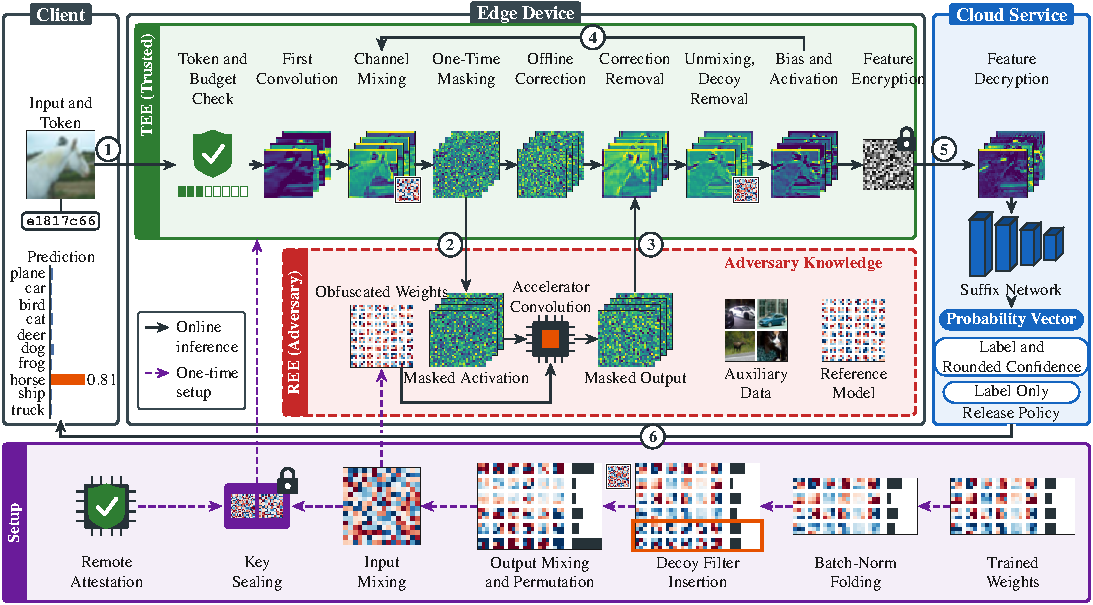
\includegraphics[width=\textwidth]{figures/ghost_architecture.pdf}
\caption{System model and workflow of GHOST}
\label{fig:architecture}
\end{figure*}

\subsection{Tier 1: Weight Obfuscation by Two-Sided Mixing with Decoys}
For each edge convolution the TEE samples $d=\lceil \delta C_o\rceil$ decoy filters $F\in\mathbb{R}^{d\times C_i\times k\times k}$ whose norms follow those of the real filters, an output mixing matrix $A\in\mathbb{R}^{(C_o+d)\times(C_o+d)}$ formed by a Haar-random orthogonal matrix scaled by random signed magnitudes, an output permutation $P$, and a Haar-random orthogonal input mixing matrix $B\in\mathbb{R}^{C_i\times C_i}$. The REE stores only
\begin{equation}
\tilde W = P\,A\begin{bmatrix}W\\ F\end{bmatrix}\big(B^{-1}\otimes I_{k^2}\big),
\label{eq:wtilde}
\end{equation}
in which the output mixing acts on the filter index and the input mixing acts on the channel index of every kernel tap. The bias $b$, the matrices $A$, $B$, $P$ and the decoys never leave the TEE. Output mixing changes the direction of every stored filter, which removes the invariant used by direction matching~\cite{wang2025arrows}. Input mixing changes the row space of the stored tensor. The decoy filters add to every stored filter a random component that is not in the span of any reference model; whether the adversary can separate it is a question that Section~\ref{sec:results} examines with explicit attacks.

\subsection{Tier 2: Masked Outsourcing of Mixed Activations}
For a layer input $a$, the TEE releases to the REE only
\begin{equation}
\tilde x = B\,a + R,\qquad R\sim\mathcal{N}\!\big(0,(\rho\,s_a)^2 I\big),
\label{eq:xtilde}
\end{equation}
where $B$ acts on the channel dimension at every spatial position, $s_a$ is the root-mean-square value of $a$ on calibration data, $\rho$ is the mask-to-signal ratio, and $R$ is drawn afresh for every request. The REE computes $\tilde y=\tilde W*\tilde x$. The correction $\tilde W*R$ is computed by the TEE in advance, during idle time, as in~\cite{tramer2018slalom,sun2023shadownet}. The TEE then recovers the pre-activation of the real filters,
\begin{equation}
W*a+b=\Big[A^{-1}P^{\top}\big(\tilde y-\tilde W*R\big)\Big]_{1:C_o}+b,
\label{eq:recover}
\end{equation}
and applies the activation function, pooling and residual additions before preparing the input of the next layer. The stored tensors and the released operands are therefore the only information about the edge prefix that the REE observes. The first convolution reads the public input, so its input-side mixing could be solved by least squares from chosen queries. GHOST executes the first convolution inside the TEE, whose cost for a $3\times3$ convolution over three input channels is negligible, and outsources only the layers whose inputs are activations that the REE never observes in plaintext.

\subsection{Tier 3: Token-Gated Execution with a Query Budget}
The model owner provisions a key $k_{\mathrm{tok}}$ in the TEE. A request for input $x$ carries a counter $c$ and a token $\tau=\mathrm{HMAC}_{k_{\mathrm{tok}}}(c\,\|\,H(x))$~\cite{krawczyk1997hmac}, where $H$ is SHA-256. A request may carry a batch of inputs, in which case $H(x)$ is the digest of the batch. The TEE serves the request only if $\tau$ verifies, $c$ exceeds the last accepted counter, and the number of inputs served so far plus the batch size does not exceed the budget $Q_{\max}$, which therefore counts inputs rather than requests. Without authorisation the TEE does not release masked operands and does not apply~\eqref{eq:recover}, so the stored tensors cannot be evaluated. Authorisation covers exactly one request.

\subsection{Tier 4: Split Execution and Output Release}
The activation at the split point is encrypted inside the TEE with AES-GCM~\cite{dworkin2007gcm} under a key $k_t$ shared with the cloud service and a fresh nonce. The cloud decrypts it, executes $f_c$, and returns the prediction according to an output release policy, which is the full probability vector, the label with its confidence rounded to one decimal, or the label alone. The suffix weights are never present on the device.

\begin{algorithm}[!t]
\caption{GHOST inference for one request}
\label{alg:ghost}
\begin{algorithmic}[1]
\Require input $x$, counter $c$, token $\tau$
\If{not $\mathrm{Verify}_{k_{\mathrm{tok}}}(c,H(x),\tau)$ \textbf{or} $c\le c_{\mathrm{last}}$ \textbf{or} $n_{\mathrm{served}}+|x|> Q_{\max}$}
  \State \Return refusal \Comment{TEE}
\EndIf
\State $c_{\mathrm{last}}\gets c$, $n_{\mathrm{served}}\gets n_{\mathrm{served}}+|x|$
\State $a\gets$ first convolution of $x$ and its activation \Comment{TEE}
\For{each outsourced convolution $\ell$}
  \State $\tilde x\gets B_\ell a+R_\ell$ \Comment{TEE}
  \State $\tilde y\gets \tilde W_\ell*\tilde x$ \Comment{REE}
  \State $z\gets [A_\ell^{-1}P_\ell^{\top}(\tilde y-M_\ell)]_{1:C_o}+b_\ell$, with $M_\ell=\tilde W_\ell*R_\ell$ precomputed \Comment{TEE}
  \State $a\gets$ activation, pooling and residual addition of $z$ \Comment{TEE}
\EndFor
\State $\gamma\gets \mathrm{AES\text{-}GCM}_{k_t}(a)$ and send $\gamma$ to the cloud \Comment{TEE}
\State \Return $\mathrm{release}(f_c(\mathrm{Dec}_{k_t}(\gamma)))$ \Comment{cloud}
\end{algorithmic}
\end{algorithm}

\section{Security Analysis}
\label{sec:analysis}

\begin{proposition}[Exactness]
\label{prop:exact}
For any input $a$, mask $R$ and secrets $(A,B,P,F)$, the value returned by~\eqref{eq:recover} equals $W*a+b$.
\end{proposition}
\begin{proof}
Convolution is linear in its input and, with zero padding, $\tilde W*(Ba+R)=\tilde W*(Ba)+\tilde W*R$. For each kernel tap the input mixing contributes the factor $B^{-1}B=I$, so $\tilde W*(Ba)=P\,A\,[W*a;\,F*a]$. Subtracting $\tilde W*R$, applying $P^{\top}$ and $A^{-1}$, and retaining the first $C_o$ channels yields $W*a$.
\end{proof}

The protected network therefore produces the same outputs as the original up to floating-point rounding. In single precision the rounding error grows with the mask ratio, because the mask is added to and subtracted from the operands, and Section~\ref{sec:results} measures the ratio up to which the predictions remain identical.

\begin{proposition}[Leakage of a masked operand]
\label{prop:mask}
Let $a\in\mathbb{R}^n$ be any random activation with $\frac{1}{n}\mathbb{E}\|a\|^2\le s_a^2$, let $B$ be orthogonal, and let $R\sim\mathcal{N}(0,\rho^2 s_a^2 I_n)$ be independent of $a$. Then
\begin{equation}
I(a;\,Ba+R)\le \frac{n}{2}\log_2\!\Big(1+\frac{1}{\rho^2}\Big)\ \text{bits}.
\end{equation}
If the same input is observed in $m$ requests with independent masks, the bound holds with $\rho^2$ replaced by $\rho^2/m$.
\end{proposition}
\begin{proof}
$B$ is invertible, so $I(a;Ba+R)=I(Ba;Ba+R)$, and $\mathbb{E}\|Ba\|^2=\mathbb{E}\|a\|^2$. For an additive Gaussian channel with average power $s_a^2$ per coordinate and noise variance $\rho^2 s_a^2$, the mutual information is at most the capacity $\frac{n}{2}\log_2(1+s_a^2/(\rho^2 s_a^2))$, which is attained by Gaussian inputs. Averaging $m$ independent observations is a sufficient statistic that reduces the noise variance by a factor $m$.
\end{proof}

With the default $\rho=10$, the bound is $\MaskBitsPerCoord$ bits per coordinate, so the first released operand of ResNet-20, the $16\times32\times32$ stem activation, carries at most $\MaskBitsImage$ bits about that activation per request, and by the data-processing inequality at most that many bits about the input; at $\rho=1000$ the figure is $\MaskBitsRhoK$ bits. The bound concerns the operands only. The adversary still observes the stored tensors, which do not depend on the input.

\begin{proposition}[Query control]
\label{prop:query}
If HMAC-SHA-256 is a pseudorandom function and the TEE counter is monotonic, an adversary that does not know $k_{\mathrm{tok}}$ and makes $q$ attempts obtains authorised executions for at most $Q_{\max}$ inputs on that device, and obtains an execution for a request that the model owner did not authorise with probability at most $q\cdot 2^{-256}+\mathrm{Adv}^{\mathrm{prf}}_{\mathrm{HMAC}}$.
\end{proposition}
\begin{proof}
The budget check and the counter are evaluated inside the TEE, so no sequence of requests exceeds $Q_{\max}$ inputs or reuses an accepted counter. Producing a valid token for a new pair $(c,H(x))$ without the key amounts to predicting an output of the pseudorandom function, which succeeds with probability $2^{-256}$ per attempt plus the PRF advantage.
\end{proof}

\begin{remark}[Stored tensors]
\label{rem:weights}
No information-theoretic claim is made for the stored tensors~\eqref{eq:wtilde}, because they are fixed and reused across requests. Permute-and-scale schemes keep the direction of every filter, which direction matching exploits~\cite{wang2025arrows}; output mixing alone keeps the row space of the stored tensor equal to the span of the real and decoy filters, onto which an adversary who knows the input transform can project a reference model. Two-sided mixing removes the known input transform, so the protection rests on the secrecy of $B$, and Section~\ref{sec:results} includes blind estimation of $B$ from the operands.
\end{remark}

\section{Experimental Setup}
\label{sec:setup}
\emph{Data.} CIFAR-10~\cite{cifar10} is divided into a member set of 40{,}000 training images on which the victim is trained, a disjoint pool of 10{,}000 training images available to the adversary as $\mathcal{D}_{\mathcal{A}}$, and the 10{,}000 test images, which serve for evaluation and as non-members.

\emph{Models.} ResNet-20~\cite{he2016resnet} and a VGG-11 network~\cite{simonyan2015vgg} with half the standard width are trained for 30 epochs with SGD, Nesterov momentum 0.9, weight decay $5\times10^{-4}$, a one-cycle learning rate with maximum 0.1, batch size 128, random cropping and horizontal flipping. The victims reach $\VicAccR\%$ (ResNet-20) and $\VicAccV\%$ (VGG-11) test accuracy. The edge prefix of ResNet-20 consists of the stem and the first three residual blocks (seven convolutions, of which the stem runs inside the TEE and six are outsourced), and the edge prefix of VGG-11 consists of the first four convolutions (one in the TEE, three outsourced). GHOST uses $\delta=0.25$ and $\rho=10$ unless stated otherwise, the signed output scales of $A$ are log-uniform in $[0.25,4]$, and the mask scale $s_a$ of each layer is calibrated on 256 images of $\mathcal{D}_{\mathcal{A}}$.

\emph{Model-stealing adversary.} The adversary initialises a network of the victim architecture, sets the edge convolutions from what it can read or recover, and fine-tunes all layers for 1{,}000 steps of SGD on $n$ images of $\mathcal{D}_{\mathcal{A}}$ with the same augmentation. The conditions are: training from scratch; the plaintext edge weights (split execution without obfuscation); the stored GHOST tensors used directly; direction matching (Hungarian assignment on sign-invariant cosine similarity with restarts, as in~\cite{wang2025arrows}); least-squares un-mixing, which fits $\tilde W_t\approx T\,W^{\mathrm{ref}}_t S$ for every kernel tap $t$ by alternating least squares and returns $T^{+}\tilde W_t S^{-1}$; and row-space projection of the reference filters onto the span of the stored filters with the input transform given to the adversary, which is an upper bound on what row-space projection can achieve from any estimate of that transform. The permute-and-scale ablation ($\tilde W=PDWQ^{\top}$) and the left-only ablation (output mixing and decoys, input channels permuted) are attacked in the same way. Two scenarios are evaluated. In the proprietary scenario the victim is trained from scratch on its member set, and the reference available to the adversary is either its own model trained on $\mathcal{D}_{\mathcal{A}}$ or an independently trained model on the victim's member set; every condition then uses the same random initialisation for the layers outside the edge prefix. In the checkpoint scenario the victim is obtained by fine-tuning for three epochs a checkpoint that the adversary also holds, and every condition starts from that checkpoint and replaces only the edge prefix. The checkpoint is a model of the same architecture trained with a different seed on the member set, so it is as close to the victim as a published checkpoint from which a deployed model has been adapted can be, and the scenario is the most favourable one for a weight-recovery attack: the checkpoint reaches $\VicAccFt\%$ before fine-tuning by the adversary. In addition to the accuracy of the fine-tuned surrogate, the relative error $\|\hat W-W\|_F/\|W\|_F$ between the recovered edge filters and the victim's folded filters is reported, averaged over the outsourced layers, together with the error of the reference model itself, which is what the adversary has without any attack.

\emph{Other adversaries.} For input reconstruction, the adversary submits 8{,}000 of its own images, records the operands released by the TEE at the first and at the last outsourced convolution, trains a convolutional decoder on these pairs for 1{,}000 steps, and applies it to 1{,}000 test images of other clients. Extraction trains a ResNet-20 surrogate on the responses to $Q$ queries drawn from $\mathcal{D}_{\mathcal{A}}$. Membership inference uses the loss~\cite{yeom2018privacy}, maximum confidence, modified entropy~\cite{song2021systematic} and label correctness~\cite{choquettechoo2021label} on 10{,}000 members and the 10{,}000 test images.

\emph{Platform.} All experiments run in PyTorch on a CPU with two threads, and timings use one thread. The TEE is simulated in the same process, so the timings characterise the relative cost of the TEE operations and the volume of data crossing the REE--TEE boundary rather than the latency of a particular device.

\section{Results}
\label{sec:results}

\subsection{Exactness}
Table~\ref{tab:exact} compares the protected and the unprotected models on the full test set for mask-to-signal ratios from 0 to $10^4$. Up to $\rho=100$ the predictions agree on every test image for both models and the relative deviation of the logits, the Frobenius norm of the logit difference over the norm of the original logits on the whole test set, is at most $\ExMaxRelErrHundred$. At $\rho=1000$ and $\rho=10^{4}$ single-precision cancellation between the mask and its correction raises the relative deviation to $1.2\times10^{-4}$ and $\ExMaxRelErr$, and the lower of the two models' agreements falls to $\ExMinAgreeK\%$ and $\ExMinAgreeTenK\%$ respectively. The ratio can therefore be raised by two orders of magnitude above the default without any change of prediction, and by three with a disagreement below 0.1\%.

\begin{table}[!t]
\centering
\caption{Exactness of the protected models}
\label{tab:exact}
\footnotesize
\setlength{\tabcolsep}{2.5pt}
\begin{tabular}{@{}lrcccc@{}}
\toprule
Model & $\rho$ & Orig.\ (\%) & GHOST (\%) & Agree.\ (\%) & Logit err. \\
\midrule
ResNet-20 & 0 & 89.94 & 89.94 & 100.00 & 4.0e-07 \\
ResNet-20 & 1 & 89.94 & 89.94 & 100.00 & 4.2e-07 \\
ResNet-20 & 10 & 89.94 & 89.94 & 100.00 & 1.2e-06 \\
ResNet-20 & 100 & 89.94 & 89.94 & 100.00 & 1.2e-05 \\
ResNet-20 & 1000 & 89.94 & 89.92 & 99.98 & 1.2e-04 \\
ResNet-20 & 10000 & 89.94 & 89.93 & 99.93 & 1.1e-03 \\
VGG-11 & 0 & 89.32 & 89.32 & 100.00 & 4.9e-07 \\
VGG-11 & 1 & 89.32 & 89.32 & 100.00 & 5.1e-07 \\
VGG-11 & 10 & 89.32 & 89.32 & 100.00 & 1.3e-06 \\
VGG-11 & 100 & 89.32 & 89.32 & 100.00 & 1.2e-05 \\
VGG-11 & 1000 & 89.32 & 89.32 & 100.00 & 1.2e-04 \\
VGG-11 & 10000 & 89.32 & 89.29 & 99.91 & 1.2e-03 \\
\bottomrule
\end{tabular}
\end{table}

\subsection{Cost}
Table~\ref{tab:overhead} reports the cost of one request at batch size 1 for three split points, in multiply-accumulate operations, which do not depend on the platform, and in measured time, as means of the components and medians of the totals over 1{,}000 requests at one thread. The original models take $\OrigMsR$~ms (ResNet-20) and $\OrigMsV$~ms (VGG-11) per request on the same thread. The online TEE work consists of the TEE-executed first convolution, input mixing and output un-mixing, and it amounts to about a quarter of the operations of the outsourced convolutions at every split except the shallowest VGG-11 split, where the TEE-executed first convolution dominates and the ratio is $0.42$, because mixing is a $1\times1$ operation at each spatial position. The REE convolution carries $1+\delta$ times the filters of the convolution it replaces, and the offline mask correction $\tilde W*R$ costs the TEE the same number of operations as the REE convolution. The total work of the TEE per request, online and offline, is therefore about $1.5$ to $1.8$ times the work of executing the outsourced prefix inside the TEE directly, and the benefit of outsourcing is confined to the latency-critical path, where the TEE performs a quarter of the operations, provided that idle time is available for the precomputation. This is the trade-off inherited from precomputed blinding~\cite{tramer2018slalom,sun2023shadownet}. The measured TEE time exceeds the REE time at every split, although the TEE performs fewer operations, because the mixing steps run as unoptimised tensor contractions in the simulation while the convolutions use the optimised library kernels. For ResNet-20 the end-to-end time of the simulated pipeline, excluding the offline correction, exceeds that of the original model by $21\%$, $64\%$ and $114\%$ at the three splits. For VGG-11 the pipeline ran faster than the single-thread baseline of the original model, which indicates a non-comparable baseline measurement rather than a property of the construction, so no end-to-end figure is reported for VGG-11. The data exchanged between the REE and the TEE per request is the volume of the released operands and of the returned results, and the activation sent to the cloud is 64~KB for a $3\times32\times32$ input, $12$~KB in single precision, at the two shallower splits of ResNet-20.

\begin{table*}[!t]
\centering
\caption{Cost of one request}
\label{tab:overhead}
\footnotesize
\setlength{\tabcolsep}{3.5pt}
\begin{tabular}{@{}lccccccccccc@{}}
\toprule
& Edge convs & \multicolumn{4}{c}{Multiply-accumulates per request (M)} & \multicolumn{4}{c}{Measured time per request (ms)} & \multicolumn{2}{c}{Data (KB)} \\\\
\cmidrule(lr){3-6}\cmidrule(lr){7-10}\cmidrule(lr){11-12}
Model & (outsourced) & Original edge & TEE online & TEE offline & REE & TEE online & REE & AES-GCM & TEE offline & REE--TEE & to cloud \\\\
\midrule
ResNet-20 & 3 (2) & 4.7 & 1.6 & 5.9 & 5.9 & 0.91 & 0.24 & 0.17 & 0.29 & 288.0 & 64.0 \\
ResNet-20 & 7 (6) & 14.2 & 4.0 & 17.7 & 17.7 & 2.09 & 0.69 & 0.18 & 0.83 & 864.0 & 64.0 \\
ResNet-20 & 14 (13) & 27.3 & 8.1 & 34.1 & 34.1 & 3.94 & 1.41 & 0.16 & 1.73 & 1432.0 & 32.0 \\
VGG-11 & 2 (1) & 4.7 & 2.5 & 5.9 & 5.9 & 0.56 & 0.15 & 0.12 & 0.18 & 112.0 & 16.0 \\
VGG-11 & 4 (3) & 18.9 & 6.4 & 23.6 & 23.6 & 1.12 & 0.66 & 0.13 & 0.73 & 240.0 & 8.0 \\
VGG-11 & 6 (5) & 33.0 & 10.3 & 41.3 & 41.3 & 1.79 & 1.43 & 0.13 & 1.54 & 304.0 & 4.0 \\
\bottomrule
\end{tabular}
\end{table*}

\subsection{Model Stealing from Device Memory}
Table~\ref{tab:steal}(a) reports the proprietary scenario with $n=5{,}000$ images. Access to the plaintext edge weights raises the surrogate from $\StealScratchR\%$ (scratch) to $\StealPlainR\%$, which quantifies the value of the protected layers to this adversary. With the stored GHOST tensors used directly the adversary reaches $\StealGhostR\%$, and the best of the adaptive attacks against GHOST reaches $\StealBestGhostR\%$, within $\StealGapR$ percentage points of training from scratch. In this scenario the reference models are unrelated to the victim at the filter level (weight error of the reference about $1.4$, the value expected for uncorrelated filters), so no weight-recovery attack has a usable reference, and the two ablations are not recovered either. The proprietary scenario therefore shows the value of the plaintext weights and the absence of any gain from the stored tensors, and the discriminating test of the obfuscation is the checkpoint scenario.


Figure~\ref{fig:stealn} shows the same comparison as a function of the size of $\mathcal{D}_{\mathcal{A}}$, with the attacks that do not use $B$ and, separately, the projection with $B$ given. The advantage of plaintext weights is largest when the adversary has little data, and the best attack on the stored GHOST tensors never exceeds training from scratch by more than $1.1$ points and falls $3$ points below it at $n=10{,}000$, in single-seed runs; direction matching and least-squares un-mixing were evaluated at $n=5{,}000$ only, and the curve at the other sizes is the better of the direct and the projection attacks. On VGG-11 with $n=5{,}000$, the corresponding figures are $\StealScratchV\%$ from scratch, $\StealPlainV\%$ with the plaintext edge weights, $\StealGhostV\%$ with the stored tensors and $\StealArrowV\%$ with direction matching against the adversary's own model.

\begin{figure}[!t]
\centering
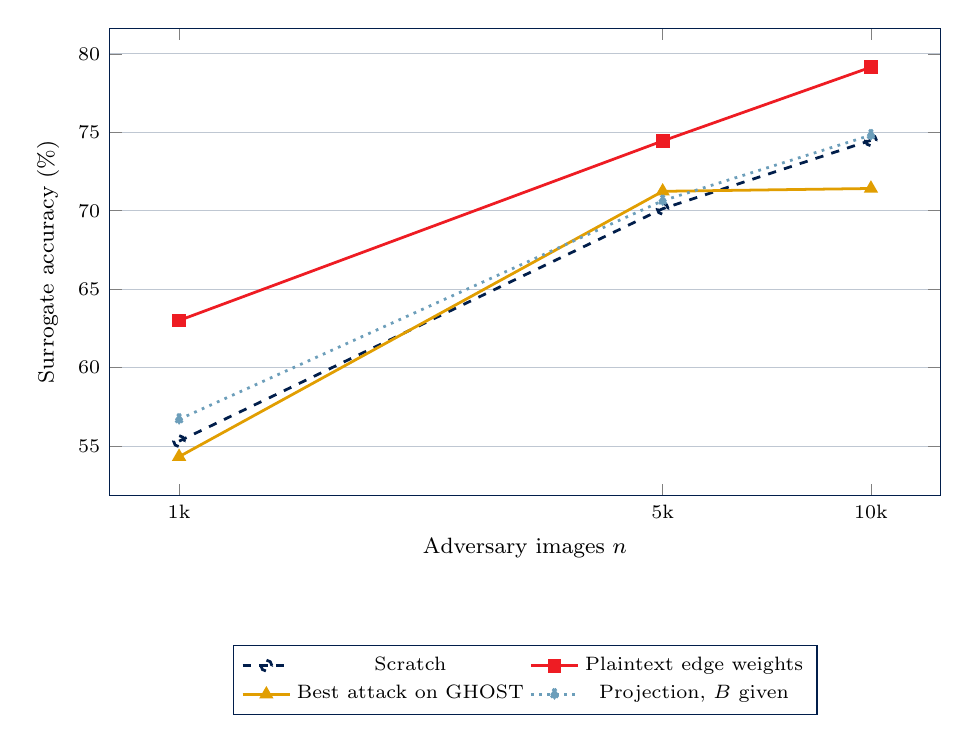
\begin{tikzpicture}
\begin{axis}[width=\columnwidth, height=0.62\columnwidth, xmode=log, xtick={1000,5000,10000},
  xticklabels={1k,5k,10k}, xlabel={Adversary images $n$}, ylabel={Surrogate accuracy (\%)},
  legend style={font=\scriptsize, at={(0.5,-0.32)}, anchor=north, draw=navy, legend columns=2},
  tick label style={font=\scriptsize}, label style={font=\footnotesize}, axis line style={navy},
  ymajorgrids, grid style={navy!25}]
\addplot[navy, mark=o, dashed, line width=1pt] coordinates {(1000,55.32) (5000,70.13) (10000,74.49)};
\addlegendentry{Scratch}
\addplot[alert, mark=square*, line width=1pt] coordinates {(1000,63.01) (5000,74.45) (10000,79.15)};
\addlegendentry{Plaintext edge weights}
\addplot[gold!90!black, mark=triangle*, very thick, line width=1pt] coordinates {(1000,54.33) (5000,71.24) (10000,71.42)};
\addlegendentry{Best attack on GHOST}
\addplot[sky!80!black, mark=diamond*, dotted, line width=1pt] coordinates {(1000,56.71) (5000,70.64) (10000,74.82)};
\addlegendentry{Projection, $B$ given}
\end{axis}
\end{tikzpicture}
\caption{Surrogate accuracy against adversary data}
\label{fig:stealn}
\end{figure}

\subsection{Checkpoint Scenario}
Table~\ref{tab:steal}(b) reports the checkpoint scenario. The checkpoint differs from the victim's folded edge filters by a relative error of $0.06$, and the adversary's fine-tuning on $\mathcal{D}_{\mathcal{A}}$ lowers its accuracy from $\VicAccFt\%$ to $\PubPublic\%$, so the accuracy column measures the damage done by fine-tuning rather than the success of an attack, and all conditions except the stored tensors used directly lie within one percentage point of it. The weight error is the operative metric and separates the conditions. Direction matching recovers the permute-and-scale ablation to an error of $\PubPsArrowErr$, below the error of the checkpoint itself, which reproduces the result of~\cite{wang2025arrows} for this class of obfuscation. Row-space projection with the input permutation given, an oracle condition, recovers the left-only ablation to $\PubLeftProjErr$. Against GHOST, direction matching and least-squares un-mixing leave errors of $\PubArrowErr$ and $\PubUnmixErr$, that is, no information about the victim's filters beyond what the checkpoint already provides, whereas projection with the true $B$ given reaches $\PubProjKErr$. The security of the stored tensors therefore rests on $B$.

\begin{table*}[!t]
\centering
\caption{Model stealing from device memory (ResNet-20, $n=5{,}000$): (a) proprietary scenario, (b) checkpoint scenario}
\label{tab:steal}
\begin{minipage}[t]{0.49\textwidth}\centering (a)\\[2pt]\footnotesize
\setlength{\tabcolsep}{3pt}
\begin{tabular}{@{}llcc@{}}
\toprule
Starting point & Ref. & Weight err. & Acc.\ (\%) \\
\midrule
Scratch & -- & -- & 70.1 \\
Plaintext edge weights & -- & -- & 74.4 \\
\midrule
GHOST tensors, direct & -- & 1.957 & 68.2 \\
GHOST, direction matching & own & 1.415 & 70.1 \\
GHOST, LS un-mixing & own & $>10$ & 67.0 \\
GHOST, direction matching & indep. & 1.423 & 71.2 \\
GHOST, LS un-mixing & indep. & $>10$ & 68.1 \\
GHOST, projection, $B$ given & indep. & 1.094 & 70.6 \\
\midrule
P\&S ablation, direction matching & indep. & 1.426 & 70.5 \\
Left-only ablation, projection & indep. & 1.094 & 70.2 \\
\bottomrule
\multicolumn{4}{@{}l@{}}{\footnotesize Weight error of the reference model alone: 1.420.}
\end{tabular}\end{minipage}\hfill
\begin{minipage}[t]{0.49\textwidth}\centering (b)\\[2pt]\footnotesize
\setlength{\tabcolsep}{3pt}
\begin{tabular}{@{}llcc@{}}
\toprule
Starting point & Ref. & Weight err. & Acc.\ (\%) \\
\midrule
Checkpoint, fine-tuned & ckpt. & -- & 86.6 \\
Plaintext edge weights & -- & -- & 86.4 \\
\midrule
GHOST tensors, direct & -- & 1.930 & 83.9 \\
GHOST, direction matching & ckpt. & 1.145 & 85.7 \\
GHOST, LS un-mixing & ckpt. & 2.789 & 86.1 \\
GHOST, projection, $B$ given & ckpt. & 0.041 & 86.8 \\
\midrule
P\&S ablation, direction matching & ckpt. & 0.029 & 86.7 \\
Left-only ablation, projection & ckpt. & 0.041 & 86.4 \\
\bottomrule
\multicolumn{4}{@{}l@{}}{\footnotesize Weight error of the reference model alone: 0.062.}
\end{tabular}\end{minipage}
\end{table*}

\subsection{Blind Estimation of the Input Mixing}
An adversary who cannot read $B$ may try to estimate it from the operands $\tilde x=Ba+R$ of its own queries, since $B$ is fixed across requests. Table~\ref{tab:ica} reports this attack for the fourth outsourced convolution of ResNet-20 ($C_i=\IcaCin$), in the checkpoint scenario. The adversary submits 2{,}000 inputs in total, which is the budget assumed in this experiment, averages $m$ repeated observations of each input, runs FastICA on the per-position channel vectors to estimate $B^{-1}$ up to row order, sign and scale, resolves the scales and the order with the per-channel activation statistics of its checkpoint, and applies the row-space projection with the estimate. Alignment is the mean over rows of $B^{-1}$ of the largest absolute cosine with an estimated row, for which the value expected from random directions is about $0.5$. The outcome depends on the effective ratio $\rho/\sqrt m$ of Proposition~\ref{prop:mask}: at $\rho=1$ with single observations, and at $\rho=10$ with $100$ repetitions of each of $20$ inputs, the rows of $B^{-1}$ are identified to an alignment of $0.95$ and $0.91$, so blind identification of the mixing is possible once the mask is averaged out, whereas at $\rho=10$ with at most $10$ repetitions and at $\rho=100$ the alignment stays close to the random value, at $0.58$ or less. Even with the identified rows the weight error after projection stays at $0.33$ and $0.40$, five to six times the error of the checkpoint, because the residual misalignment and the scale errors are amplified by the projection; the best error over all settings, $\IcaBestErr$, compares with $\IcaTrueB$ for the true $B$ and $\IcaRefErr$ for the checkpoint alone at this layer, which differs from the $0.062$ of Table~\ref{tab:steal}(b) because the latter is the mean over the outsourced layers. A refinement of the ICA estimate by continuous optimisation on the orthogonal group was not implemented and may narrow this gap. The parameters that limit the attack are therefore the mask ratio and the budget: with $Q_{\max}$ inputs an adversary can obtain $m\le Q_{\max}/C_i$ repetitions of enough inputs for the estimate, and keeping $\rho/\sqrt{Q_{\max}}$ at or above $3$, the value at which the alignment stayed close to the random value, costs nothing in accuracy up to $\rho=100$ and less than $0.1\%$ of the predictions up to $\rho=10^4$ (Table~\ref{tab:exact}).

\begin{table}[!t]
\centering
\caption{Blind estimation of $B$ from released operands (ResNet-20, fourth outsourced convolution)}
\label{tab:ica}
\footnotesize
\setlength{\tabcolsep}{4pt}
\begin{tabular}{@{}cccccc@{}}
\toprule
$\rho$ & Repeats $m$ & Inputs & Alignment & \multicolumn{2}{c}{Weight error after projection} \\
\cmidrule(l){5-6}
& & & & ICA estimate & with reference scales \\
\midrule
1 & 1 & 2000 & 0.95 & 0.651 & 0.329 \\
10 & 1 & 2000 & 0.51 & 0.805 & 0.793 \\
10 & 10 & 200 & 0.58 & 0.841 & 0.721 \\
10 & 100 & 20 & 0.91 & 0.748 & 0.400 \\
100 & 10 & 200 & 0.52 & 0.834 & 0.835 \\
100 & 100 & 20 & 0.50 & 0.818 & 0.787 \\
\bottomrule
\end{tabular}
\end{table}

\subsection{Input Reconstruction}
Table~\ref{tab:inversion} reports the reconstruction quality of the decoder for the operands of the first and the last outsourced convolution. Without masking ($\rho=0$) the operand of the first outsourced layer is a channel-mixed copy of the stem activation, and the decoder reconstructs the input from it with a peak signal-to-noise ratio (PSNR) of $\InvPsnrFirstZero$~dB. With $\rho=10$ the PSNR falls to $\InvPsnrFirstTen$~dB, close to that of predicting the mean image of the dataset ($\InvPsnrMean$~dB). Figure~\ref{fig:inversion} shows reconstructions for both settings. The trusted cloud receives the unmasked split activation, which lies three operations beyond the last operand of Table~\ref{tab:inversion}, so the input is reconstructible from it at approximately the PSNR of the last-layer row with $\rho=0$, and the privacy of the input with respect to the cloud is that of split inference.

\begin{table}[!t]
\centering
\caption{Input reconstruction from released operands (ResNet-20)}
\label{tab:inversion}
\footnotesize
\begin{tabular}{@{}lccc@{}}
\toprule
Observed operand & $\rho$ & PSNR (dB) & SSIM \\
\midrule
First outsourced conv. & 0 & 37.18 & 0.991 \\
Last outsourced conv. & 0 & 21.00 & 0.791 \\
First outsourced conv. & 1 & 24.58 & 0.839 \\
Last outsourced conv. & 1 & 16.87 & 0.655 \\
First outsourced conv. & 10 & 13.36 & 0.200 \\
Last outsourced conv. & 10 & 12.76 & 0.169 \\
First outsourced conv. & 100 & 12.62 & 0.123 \\
Last outsourced conv. & 100 & 12.63 & 0.121 \\
\midrule
Mean image of $\mathcal{D}_{\mathcal{A}}$ & -- & 12.70 & 0.128 \\
\bottomrule
\end{tabular}
\end{table}

\begin{figure}[!t]
\centering
\subfloat[$\rho=0$]{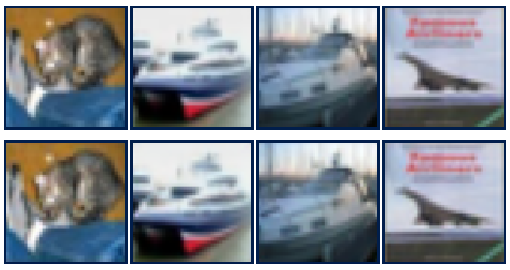
\includegraphics[width=0.48\columnwidth]{generated/inv_rho0.pdf}}\hfill
\subfloat[$\rho=10$]{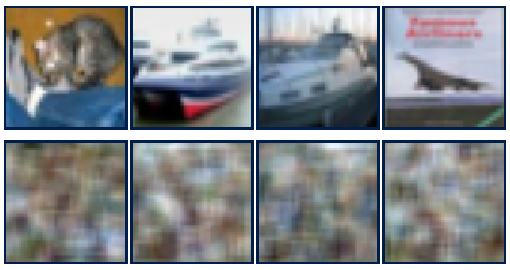
\includegraphics[width=0.48\columnwidth]{generated/inv_rho10.pdf}}
\caption{Reconstructions from the operands of the first outsourced layer}
\label{fig:inversion}
\end{figure}

\subsection{Query-Based Extraction}
Figure~\ref{fig:extract} reports the accuracy of a surrogate trained on the responses to $Q$ authorised queries. Because GHOST is exact, a surrogate trained on a given number of responses is as accurate as one trained against the unprotected model, and the protection against this attack is the budget $Q_{\max}$ enforced by Proposition~\ref{prop:query}. Label-only release lowers the accuracy reached for a given budget.

\begin{figure}[!t]
\centering
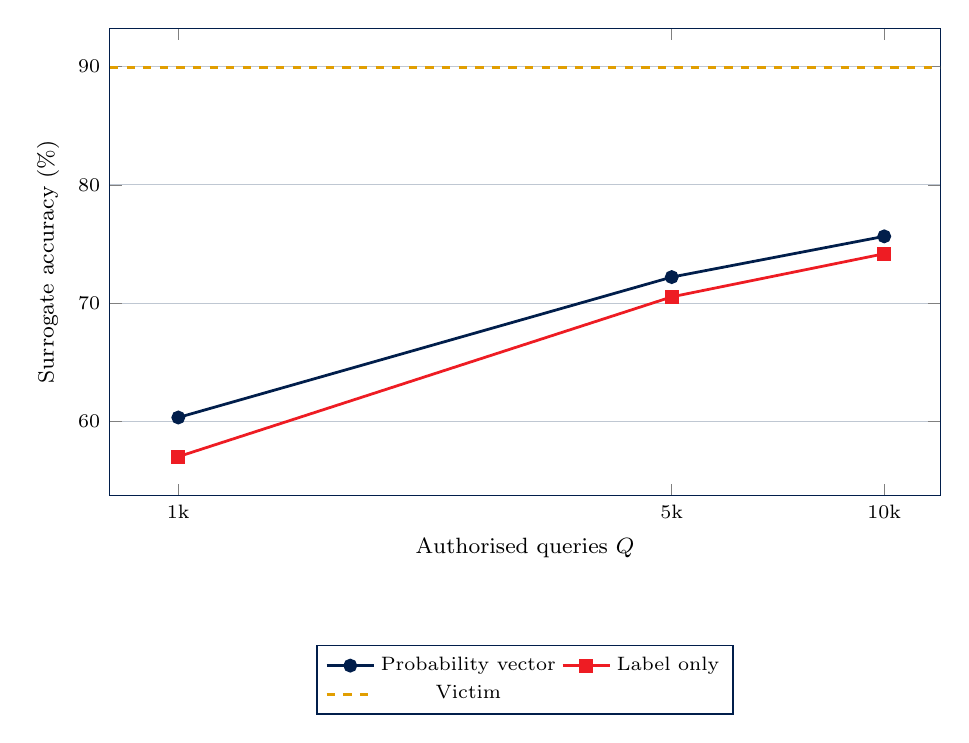
\begin{tikzpicture}
\begin{axis}[width=\columnwidth, height=0.62\columnwidth, xmode=log, xtick={1000,5000,10000},
  xticklabels={1k,5k,10k}, xlabel={Authorised queries $Q$}, ylabel={Surrogate accuracy (\%)},
  legend style={font=\scriptsize, at={(0.5,-0.32)}, anchor=north, draw=navy, legend columns=2},
  tick label style={font=\scriptsize}, label style={font=\footnotesize}, axis line style={navy},
  ymajorgrids, grid style={navy!25}, xmin=800, xmax=12000]
\addplot[navy, mark=*, line width=1pt] coordinates {(1000,60.35) (5000,72.21) (10000,75.65)};
\addlegendentry{Probability vector}
\addplot[alert, mark=square*, line width=1pt] coordinates {(1000,57.04) (5000,70.54) (10000,74.18)};
\addlegendentry{Label only}
\addplot[gold!90!black, dashed, line width=1pt, domain=800:12000, samples=2] {89.94};
\addlegendentry{Victim}
\end{axis}
\end{tikzpicture}
\caption{Extraction accuracy against query budget}
\label{fig:extract}
\end{figure}

\subsection{Membership Inference}
Table~\ref{tab:mia} reports the area under the ROC curve (AUC) of four membership inference attacks under the three output release policies. The protected and the unprotected models give identical values, as Proposition~\ref{prop:exact} implies, so GHOST neither adds nor removes membership leakage. For this victim, whose training and test accuracies are $95.6\%$ and $89.9\%$, all four attacks are close to chance, with an AUC of at most $0.536$, and the release policies change the AUC by at most $0.027$, for the confidence attack under label-only release, which removes the score it uses. The likelihood-ratio attack~\cite{carlini2022lira}, which requires shadow models, was not run.

\begin{table}[!t]
\centering
\caption{Membership inference AUC (ResNet-20)}
\label{tab:mia}
\footnotesize
\setlength{\tabcolsep}{3pt}
\begin{tabular}{@{}llcccc@{}}
\toprule
Release policy & Model & Loss & Conf. & Mod.\ entropy & Correctness \\
\midrule
Probability vector & Original & 0.529 & 0.522 & 0.529 & 0.529 \\
 & GHOST & 0.529 & 0.522 & 0.529 & 0.529 \\
Label + rounded conf. & Original & 0.536 & 0.527 & 0.535 & 0.529 \\
 & GHOST & 0.536 & 0.527 & 0.535 & 0.529 \\
Label only & Original & 0.529 & 0.500 & 0.526 & 0.529 \\
 & GHOST & 0.529 & 0.500 & 0.526 & 0.529 \\
\bottomrule
\end{tabular}
\end{table}

\subsection{Token-Gated Execution}
Table~\ref{tab:token} lists the response of the TEE to a sequence of requests with a budget of five. Replayed tokens, tokens bound to a different input, forged tokens and direct execution of the stored tensors without authorisation are refused, and service stops once the budget is exhausted.

\begin{table}[!t]
\centering
\caption{Responses of the token gate (budget $Q_{\max}=5$)}
\label{tab:token}
\footnotesize
\begin{tabular}{@{}lc@{}}
\toprule
Request & TEE response \\
\midrule
Valid token, fresh counter & Served \\
Replay of the same token and counter & Refused \\
Valid token reused for a different input & Refused \\
Forged token (random 256-bit string) & Refused \\
Protected pipeline run without authorisation & Refused \\
Valid token, counter 4 (budget 5) & Served \\
Valid token, counter 5 (budget 5) & Served \\
Valid token, counter 6 (budget 5) & Served \\
Valid token, counter 7 (budget 5) & Served \\
Valid token, counter 8 (budget 5) & Refused \\
Valid token, counter 9 (budget 5) & Refused \\
Valid token, counter 10 (budget 5) & Refused \\
Valid token, counter 11 (budget 5) & Refused \\
\bottomrule
\end{tabular}
\end{table}

\section{Discussion and Limitations}
\label{sec:discussion}
The TEE is simulated in software, so the measured times do not include the cost of world switches on a TrustZone device or the reduced throughput of enclave code; the operation counts and the data volumes per request are independent of the platform and are reported for this reason, and a deployment on a development board with OP-TEE is necessary to establish the latency on real hardware. Token issuance requires the model owner to be reachable at request time and to see the digest of every input, and the budget is enforced per device, so an adversary who controls several devices or token allocations multiplies $Q_{\max}$ accordingly. The online TEE cost of mixing and recovery grows with the square of the channel count, which is why GHOST places only the first stages of the network on the device and the suffix in the cloud; depthwise convolutions, as used in MobileNet architectures, require a channel-wise variant of~\eqref{eq:wtilde}.

With $B$ given, row-space projection recovers the filters. The adaptive attacks of Section~\ref{sec:results}, including blind estimation of $B$ from the operands, are the strongest procedures implemented in this study, and stronger attacks may exist. The mask ratio and the query budget limit blind estimation, since $m$ repeated observations reduce the effective ratio by $\sqrt m$ (Proposition~\ref{prop:mask}); the ratio can be raised to $100$ without any change of prediction and to $10^4$ with a disagreement below $0.1\%$. Membership inference through the returned predictions is not affected by the weight and operand protections and is addressed by the output release policy.

\section{Conclusion}
\label{sec:conclusion}
This paper presented GHOST, a TEE-anchored construction for edge inference that protects the weights in device memory by two-sided mixing with decoy filters, the released operands by one-time masking, and the query interface by token-gated execution with a budget, and keeps the suffix of the network in the cloud. The construction is exact and preserved the predictions of ResNet-20 and VGG-11 on every CIFAR-10 test image at the default mask ratio. In an adaptive evaluation, the stored tensors gave a device-level adversary no advantage beyond one percentage point over training from scratch in single-seed runs and no information beyond a related checkpoint, whereas the permute-and-scale and left-only ablations were recovered; blind estimation of the input mixing identified its rows only at a low effective mask ratio, which the mask ratio and the query budget control. Masked operands reduced input reconstruction to close to an uninformed guess, and extraction was bounded by the enforced budget.

\begin{thebibliography}{99}
\bibitem{tramer2016stealing}
F. Tram\`{e}r, F. Zhang, A. Juels, M. K. Reiter, and T. Ristenpart, ``Stealing machine learning models via prediction APIs,'' in \emph{Proc. 25th USENIX Security Symp.}, 2016, pp. 601--618.

\bibitem{orekondy2019knockoff}
T. Orekondy, B. Schiele, and M. Fritz, ``Knockoff nets: Stealing functionality of black-box models,'' in \emph{Proc. IEEE/CVF Conf. Comput. Vis. Pattern Recognit. (CVPR)}, 2019, pp. 4954--4963.

\bibitem{shokri2017membership}
R. Shokri, M. Stronati, C. Song, and V. Shmatikov, ``Membership inference attacks against machine learning models,'' in \emph{Proc. IEEE Symp. Security and Privacy (SP)}, 2017, pp. 3--18.

\bibitem{carlini2022lira}
N. Carlini, S. Chien, M. Nasr, S. Song, A. Terzis, and F. Tram\`{e}r, ``Membership inference attacks from first principles,'' in \emph{Proc. IEEE Symp. Security and Privacy (SP)}, 2022, pp. 1897--1914.

\bibitem{pinto2019trustzone}
S. Pinto and N. Santos, ``Demystifying Arm TrustZone: A comprehensive survey,'' \emph{ACM Comput. Surv.}, vol. 51, no. 6, pp. 1--36, 2019.

\bibitem{mo2020darknetz}
F. Mo, A. S. Shamsabadi, K. Katevas, S. Demetriou, I. Leontiadis, A. Cavallaro, and H. Haddadi, ``DarkneTZ: Towards model privacy at the edge using trusted execution environments,'' in \emph{Proc. 18th Int. Conf. Mobile Syst., Appl., Services (MobiSys)}, 2020, pp. 161--174.

\bibitem{zhang2024nplo}
Z. Zhang, C. Gong, Y. Cai, Y. Yuan, B. Liu, D. Li, Y. Guo, and X. Chen, ``No privacy left outside: On the (in-)security of TEE-shielded DNN partition for on-device ML,'' in \emph{Proc. IEEE Symp. Security and Privacy (SP)}, 2024, pp. 3327--3345.

\bibitem{tramer2018slalom}
F. Tram\`{e}r and D. Boneh, ``Slalom: Fast, verifiable and private execution of neural networks in trusted hardware,'' in \emph{Proc. Int. Conf. Learn. Represent. (ICLR)}, 2019.

\bibitem{sun2023shadownet}
Z. Sun, R. Sun, C. Liu, A. Roy Chowdhury, L. Lu, and S. Jha, ``ShadowNet: A secure and efficient on-device model inference system for convolutional neural networks,'' in \emph{Proc. IEEE Symp. Security and Privacy (SP)}, 2023, pp. 1596--1612.

\bibitem{shen2022soter}
T. Shen, J. Qi, J. Jiang, X. Wang, S. Wen, X. Chen, S. Zhao, S. Wang, L. Chen, X. Luo, F. Zhang, and H. Cui, ``SOTER: Guarding black-box inference for general neural networks at the edge,'' in \emph{Proc. USENIX Annu. Tech. Conf. (ATC)}, 2022, pp. 723--738.

\bibitem{zhang2024groupcover}
Z. Zhang, N. Wang, Z. Zhang, Y. Zhang, T. Zhang, J. Liu, and Y. Wu, ``GroupCover: A secure, efficient and scalable inference framework for on-device model protection based on TEEs,'' in \emph{Proc. 41st Int. Conf. Mach. Learn. (ICML)}, PMLR vol. 235, 2024, pp. 59992--60003.

\bibitem{sun2025tsqp}
Y. Sun, G. Xiong, J. Liu, Z. Liu, and J. Cui, ``TSQP: Safeguarding real-time inference for quantization neural networks on edge devices,'' in \emph{Proc. IEEE Symp. Security and Privacy (SP)}, 2025, pp. 2114--2132.

\bibitem{wang2025arrows}
P. Wang, B. Dong, Y. Cai, Z. Zhang, J. Liu, H. Xue, Y. Wu, Y. Zhang, and Z. Zhang, ``Game of arrows: On the (in-)security of weight obfuscation for on-device TEE-shielded LLM partition algorithms,'' in \emph{Proc. 34th USENIX Security Symp.}, 2025, pp. 279--298.

\bibitem{mao2025amulet}
Z. Mao, L. Zhao, L. Xu, W. Dong, S. Zhang, C. Wang, and Q. Wang, ``Amulet: Fast TEE-shielded inference for on-device model protection,'' \emph{arXiv preprint arXiv:2512.07495}, 2025.

\bibitem{zhou2023nnsplitter}
T. Zhou, Y. Luo, S. Ren, and X. Xu, ``NNSplitter: An active defense solution for DNN model via automated weight obfuscation,'' in \emph{Proc. 40th Int. Conf. Mach. Learn. (ICML)}, PMLR vol. 202, 2023, pp. 42614--42624.

\bibitem{zheng2026miragenet}
H. Zheng, L. Cheng, and Y. Ding, ``MirageNet: A secure, efficient, and scalable on-device model protection in heterogeneous TEE and GPU system,'' \emph{arXiv preprint arXiv:2601.13826}, 2026.

\bibitem{oliynyk2023survey}
D. Oliynyk, R. Mayer, and A. Rauber, ``I know what you trained last summer: A survey on stealing machine learning models and defences,'' \emph{ACM Comput. Surv.}, vol. 55, no. 14s, pp. 1--41, 2023.

\bibitem{yeom2018privacy}
S. Yeom, I. Giacomelli, M. Fredrikson, and S. Jha, ``Privacy risk in machine learning: Analyzing the connection to overfitting,'' in \emph{Proc. IEEE 31st Comput. Security Found. Symp. (CSF)}, 2018, pp. 268--282.

\bibitem{song2021systematic}
L. Song and P. Mittal, ``Systematic evaluation of privacy risks of machine learning models,'' in \emph{Proc. 30th USENIX Security Symp.}, 2021, pp. 2615--2632.

\bibitem{choquettechoo2021label}
C. A. Choquette-Choo, F. Tram\`{e}r, N. Carlini, and N. Papernot, ``Label-only membership inference attacks,'' in \emph{Proc. 38th Int. Conf. Mach. Learn. (ICML)}, PMLR vol. 139, 2021, pp. 1964--1974.

\bibitem{song2019memguard}
J. Jia, A. Salem, M. Backes, Y. Zhang, and N. Z. Gong, ``MemGuard: Defending against black-box membership inference attacks via adversarial examples,'' in \emph{Proc. ACM SIGSAC Conf. Comput. Commun. Security (CCS)}, 2019, pp. 259--274.

\bibitem{tang2024modelguard}
M. Tang, A. Dai, L. DiValentin, A. Ding, A. Hass, N. Z. Gong, and Y. Chen, ``ModelGuard: Information-theoretic defense against model extraction attacks,'' in \emph{Proc. 33rd USENIX Security Symp.}, 2024, pp. 5305--5322.

\bibitem{pang2025modelshield}
K. Pang, T. Qi, C. Wu, M. Bai, M. Jiang, and Y. Huang, ``ModelShield: Adaptive and robust watermark against model extraction attack,'' \emph{IEEE Trans. Inf. Forensics Security}, vol. 20, pp. 1767--1782, 2025.

\bibitem{thapa2022splitfed}
C. Thapa, P. C. M. Arachchige, S. Camtepe, and L. Sun, ``SplitFed: When federated learning meets split learning,'' in \emph{Proc. AAAI Conf. Artif. Intell.}, vol. 36, no. 8, 2022, pp. 8485--8493.

\bibitem{he2019inversion}
Z. He, T. Zhang, and R. B. Lee, ``Model inversion attacks against collaborative inference,'' in \emph{Proc. 35th Annu. Comput. Security Appl. Conf. (ACSAC)}, 2019, pp. 148--162.

\bibitem{batina2018csi}
L. Batina, S. Bhasin, D. Jap, and S. Picek, ``CSI NN: Reverse engineering of neural network architectures through electromagnetic side channel,'' in \emph{Proc. 28th USENIX Security Symp.}, 2019, pp. 515--532.

\bibitem{yan2020cachetelepathy}
M. Yan, C. W. Fletcher, and J. Torrellas, ``Cache telepathy: Leveraging shared resource attacks to learn DNN architectures,'' in \emph{Proc. 29th USENIX Security Symp.}, 2020, pp. 2003--2020.

\bibitem{horvath2024sok}
P. Horv\'{a}th, D. Lauret, Z. Liu, and L. Batina, ``SoK: Neural network extraction through physical side channels,'' in \emph{Proc. 33rd USENIX Security Symp.}, 2024.

\bibitem{gilad2016cryptonets}
R. Gilad-Bachrach, N. Dowlin, K. Laine, K. Lauter, M. Naehrig, and J. Wernsing, ``CryptoNets: Applying neural networks to encrypted data with high throughput and accuracy,'' in \emph{Proc. 33rd Int. Conf. Mach. Learn. (ICML)}, PMLR vol. 48, 2016, pp. 201--210.

\bibitem{rathee2020cryptflow2}
D. Rathee, M. Rathee, N. Kumar, N. Chandran, D. Gupta, A. Rastogi, and R. Sharma, ``CrypTFlow2: Practical 2-party secure inference,'' in \emph{Proc. ACM SIGSAC Conf. Comput. Commun. Security (CCS)}, 2020, pp. 325--342.

\bibitem{dworkin2007gcm}
M. Dworkin, ``Recommendation for block cipher modes of operation: Galois/counter mode (GCM) and GMAC,'' Nat. Inst. Standards Technol., NIST Special Publication 800-38D, 2007.

\bibitem{krawczyk1997hmac}
H. Krawczyk, M. Bellare, and R. Canetti, ``HMAC: Keyed-hashing for message authentication,'' IETF RFC 2104, 1997.

\bibitem{cifar10}
A. Krizhevsky, ``Learning multiple layers of features from tiny images,'' Univ. Toronto, Tech. Rep., 2009.

\bibitem{he2016resnet}
K. He, X. Zhang, S. Ren, and J. Sun, ``Deep residual learning for image recognition,'' in \emph{Proc. IEEE Conf. Comput. Vis. Pattern Recognit. (CVPR)}, 2016, pp. 770--778.

\bibitem{simonyan2015vgg}
K. Simonyan and A. Zisserman, ``Very deep convolutional networks for large-scale image recognition,'' in \emph{Proc. Int. Conf. Learn. Represent. (ICLR)}, 2015.
\end{thebibliography}

\vspace{-2em}
\begin{IEEEbiography}[{
\includegraphics[width=1in,height=1.25in,clip,keepaspectratio]{sidd.jpeg}}]{Siddharath Malavalli Nagesh}
received the B.E.\ degree in Computer Science from Birla Institute of Technology and Science, Pilani, in 2026. During his undergraduate studies, he focused on machine learning systems security, with particular emphasis on adversarial robustness and privacy-preserving inference for edge-deployed neural networks. He is the lead developer of the GHOST framework, responsible for the implementation of the defence pipeline, the attack suite, and the multi-architecture training infrastructure. His research interests include edge AI security, model extraction defences, and cryptographic approaches to neural network protection.
\end{IEEEbiography}

\begin{IEEEbiography}[{
\includegraphics[width=1in,height=1.25in,clip,keepaspectratio]{firas.jpeg}}]{Mohamed Firas Adil}
received the B.E.\ degree in Computer Science from Birla Institute of Technology and Science, Pilani, in 2025. He is currently an Engineer with the EQS Department, Siemens Energy, Expo City, Dubai, UAE, where he works on secure data acquisition and edge computing systems for industrial energy infrastructure. He contributed the initial training scaffolding and baseline evaluation code for the GHOST project during his undergraduate studies. His research interests include industrial IoT security, secure inference for operational technology environments, and privacy-preserving machine learning for edge systems deployed in safety-critical industrial settings.
\end{IEEEbiography}

\begin{IEEEbiography}[{
\includegraphics[width=1in,height=1.25in,clip,keepaspectratio]{rochi.jpeg}}]{Rochishnu Banerjee}
is pursuing the B.S.\ degree in Computer Science and Software Engineering at Miami University, Oxford, OH, USA. His undergraduate research focuses on the intersection of software security and machine learning, with specific interest in adversarial attacks against deployed AI systems and the formal analysis of defence mechanisms. He contributed to the theoretical analysis and evaluation methodology of the GHOST framework. His research interests include software security, adversarial machine learning, secure system design, and the application of formal methods to the verification of AI system security properties.
\end{IEEEbiography}

\begin{IEEEbiography}[{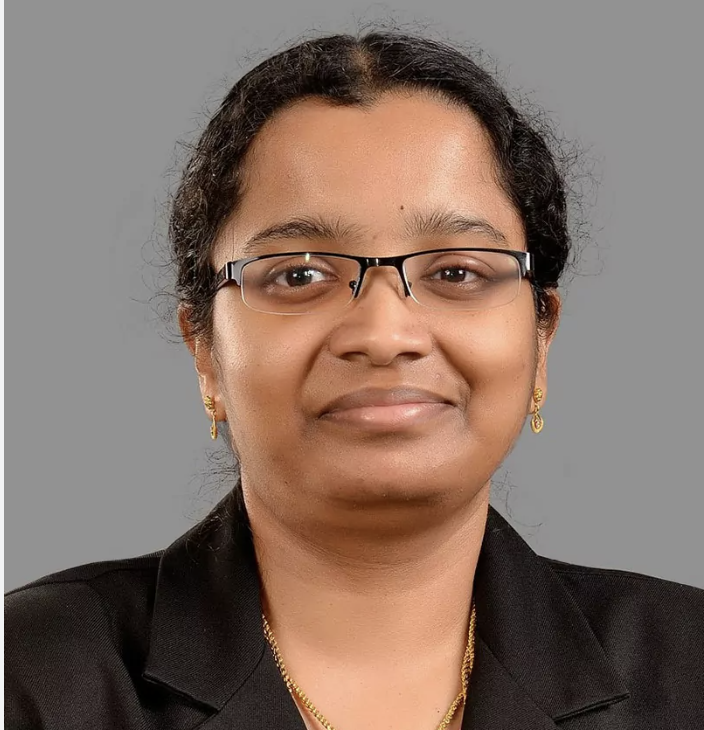
\includegraphics[width=1in,height=1.25in,clip,keepaspectratio]{angel.png}}]{Angel Arul Jothi Joseph}
received the B.E.\ degree in Computer Science and Engineering from Madras University in 2004, the M.Tech.\ degree in Information Technology from College of Engineering Guindy, Anna University, Chennai, India, in 2011, and the Ph.D.\ degree in Computer Science and Engineering from Anna University in 2017. Since 2017, she has been an Assistant Professor with the Department of Computer Science, Birla Institute of Technology and Science, Pilani, Dubai Campus, Dubai, UAE. Her research interests include image processing, computer vision, deep learning, bioinformatics, and natural language processing. She has published more than 50 journal and conference papers and supervised doctoral and postgraduate research. (ORCID: 0000-0002-1773-8779)
\end{IEEEbiography}

\begin{IEEEbiography}[{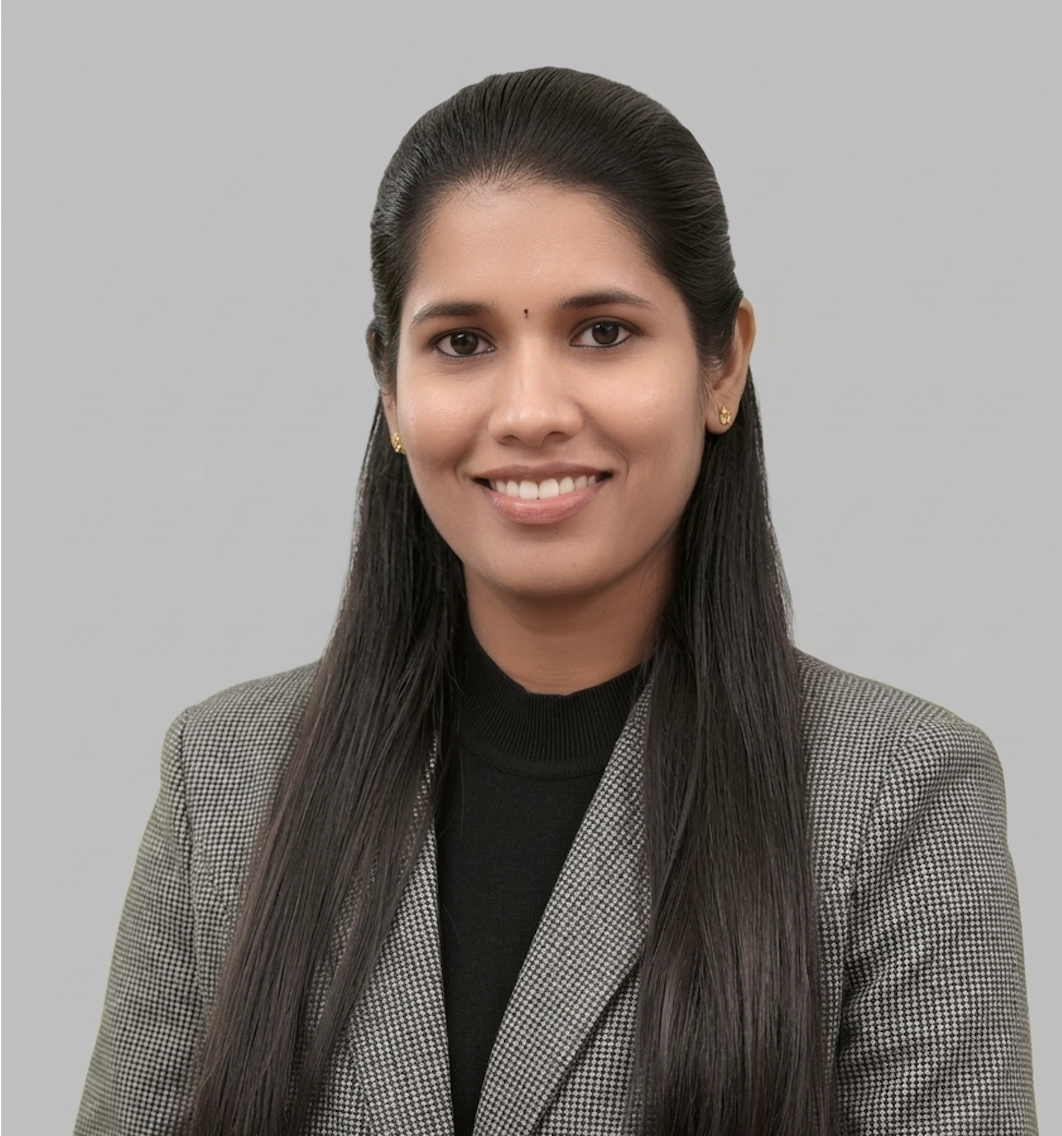
\includegraphics[width=1in,height=1.25in,clip,keepaspectratio]{elakkiya.png}}]{Elakkiya Rajasekar}
received the B.E.\ degree in Computer Science and Engineering, the M.E.\ degree in Software Engineering, and the Ph.D.\ degree, all from Anna University, Chennai, India, in 2010, 2012, and 2018, respectively. She is currently an Associate Professor with the Department of Computer Science, Birla Institute of Technology and Science, Pilani, Dubai Campus, Dubai International Academic City, Dubai, UAE, and serves as Associate Head of the Anuradha and Prashanth Palakurthi Centre for Artificial Intelligence Research (APPCAIR). She has published more than 95 research articles in IEEE Transactions, Elsevier, and Springer venues, holds 6 patents, and has authored 12 books and 12 book chapters. She has been recognised among the Top 2\% World Scientists by the Stanford--Elsevier global rankings (2024--25 and 2025--26). She serves as Chair of the ACM-W Professional Dubai Chapter and Vice President of the ACM Dubai Professional Chapter. Her research interests include edge AI security, privacy-preserving machine learning, adversarial robustness, and sign language recognition. She is the corresponding author of this paper. (ORCID: 0000-0002-2257-0640)
\end{IEEEbiography}

\end{document}
